% !TeX spellcheck = pt_PT

\chapter{Validação e Testes}
\label{ch:validacaoTestes}

A validação do sistema desenvolvido foi conduzida de forma incremental, começando por testes unitários a cada componente de \emph{hardware}, passando pela integração em ambiente controlado e culminando na experimentação em cenários reais. Esta abordagem permitiu não apenas garantir o correto funcionamento de cada subsistema de forma isolada, mas também identificar precocemente potenciais falhas de integração, reduzindo o risco de insucesso em fases mais avançadas.  

\section{Testes Incrementais de \emph{Hardware}}

Antes da integração completa no protótipo do \gls{usv}, foram realizados testes individuais a cada módulo de \emph{hardware}, recorrendo a programas de validação dedicados. Estes testes encontram-se documentados no repositório público associado a este projeto \cite{github-usv}, na diretoria \texttt{examples}. Cada exemplo foi concebido para verificar a operação de um subsistema específico, assegurando que todos os módulos funcionavam corretamente de forma isolada.  

No caso do \gls{imu}, foi implementada uma leitura contínua das acelerações, rotações e campo magnético, permitindo validar a calibração inicial e a estabilidade dos valores registados. Para o módulo \gls{gps} BN-880, procedeu-se à descodificação de mensagens \gls{nmea} e à aquisição de coordenadas em tempo real, confirmando tanto a receção de satélites como a fiabilidade da posição estimada. Relativamente aos propulsores, foram gerados sinais \gls{pwm} direcionados aos \gls{esc}, testando o processo de armamento e a resposta do sistema a diferentes larguras de pulso.  

A comunicação \gls{lora} foi também alvo de verificação, com o envio e receção de mensagens simples que permitiram avaliar a estabilidade do canal e a correta configuração do transceptor. Por fim, o \emph{display} \gls{oled} integrado foi utilizado para apresentar mensagens de \emph{debug}, demonstrando a sua utilidade na monitorização em tempo real da receção de dados provenientes dos sensores.  

Estes ensaios confirmaram o funcionamento básico de todos os módulos de forma independente, assegurando que as interfaces de comunicação (\gls{i2c}, \gls{uart}, \gls{pwm}) e as camadas de abstração implementadas estavam operacionais antes da integração no sistema completo.

\section{Integração e Testes de Sistema}

Após a validação individual de cada componente, procedeu-se à integração progressiva do sistema. Inicialmente, os propulsores foram testados em conjunto, verificando a coerência do movimento diferencial e a execução de manobras básicas (frente, trás e rotações). Posteriormente, o \gls{imu} e o \gls{gps} foram integrados com o sistema de controlo, validando a fusão de dados de orientação e navegação com a lógica de \emph{waypoints}.  

Em paralelo, a comunicação \gls{lora} foi testada para garantir a transmissão de telemetria e a receção de comandos remotos, sem comprometer o funcionamento do ciclo principal. A utilização de mensagens estruturadas com \emph{Protobuf} demonstrou vantagens significativas na redução do tempo de transmissão e na fiabilidade da comunicação.  

Todos os ensaios desta fase foram realizados em ambiente controlado de laboratório, permitindo afinar parâmetros de \emph{software} e validar a robustez da implementação antes da realização de testes em condições reais.  

\section{Validação em Ambiente Real}

A validação final do sistema ocorreu no âmbito do exercício internacional \gls{repmus25}, considerado o maior exercício mundial de robótica marítima \cite{iddportugal-repmus, sapo-repmus}. O protótipo desenvolvido foi testado no subevento \gls{rex25}, organizado pela Escola Naval \cite{escolanaval-repmus}, que visa promover a experimentação tecnológica e a cooperação em cenários operacionais simulados, no contexto das operações não tripuladas.  

Este teste constituiu um marco relevante na validação do sistema, uma vez que permitiu avaliar o desempenho do \gls{usv} em condições operacionais reais, incluindo a comunicação de longo alcance via \gls{lora} e a execução de rotas predefinidas com recurso ao \gls{gps} e ao \gls{imu}.  

A participação no \gls{rex25}, integrado no \gls{repmus25}, demonstrou a aplicabilidade prática da solução desenvolvida e reforçou o contributo da Escola Náutica e da investigação nacional no domínio dos sistemas ciberfísicos aplicados à robótica marítima. Esta validação permitiu comprovar a robustez, escalabilidade e relevância prática do sistema, consolidando o trabalho desenvolvido no âmbito desta \gls{tfm}.

Durante o processo de validação identificou-se a necessidade de complementar os testes com uma ferramenta de apoio à visualização geográfica dos \emph{waypoints}, de forma a avaliar em tempo real a coerência e a precisão das rotas definidas. Para tal, foi desenvolvida uma aplicação em \gls{html} que, recorrendo a um servidor de \emph{map tiling}, permite representar graficamente a posição geográfica de cada \emph{waypoint} no globo. Esta ferramenta revelou-se essencial para a interpretação e validação prática das trajetórias, uma vez que forneceu uma perspetiva espacial clara do percurso programado e da sua correspondência com o ambiente real.  

Para além da sua utilidade imediata na fase de testes, esta aplicação possui elevado potencial para ser expandida em trabalhos futuros, nomeadamente através da integração com sistemas de monitorização remota, planeamento dinâmico de rotas e visualização em tempo real do estado do \gls{usv}. Desta forma, poderá constituir-se como um módulo complementar para a exploração e gestão de missões autónomas em cenários operacionais complexos.  

A Figura~\ref{fig:html} apresenta uma captura de ecrã da aplicação desenvolvida, evidenciando a sua utilidade como suporte complementar à experimentação em campo.


\begin{figure}[H]
    \centering
    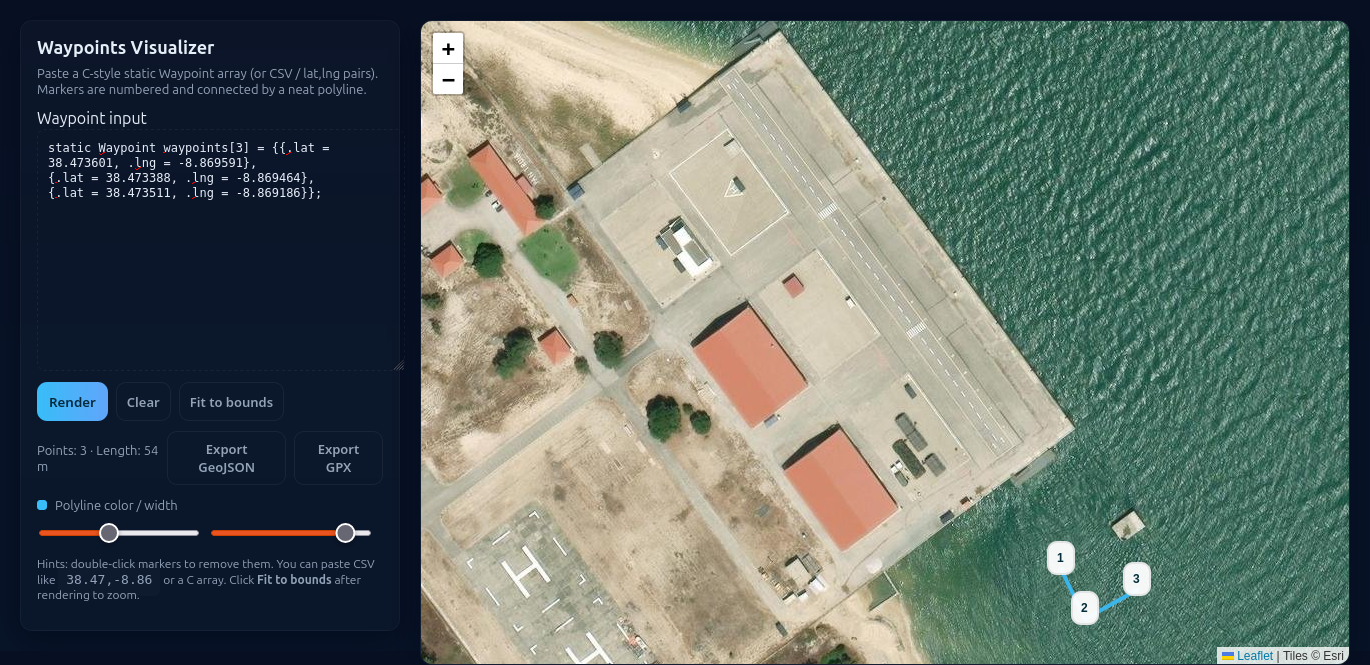
\includegraphics[width=1\linewidth]{figuras/waypoint-html.png}
    \caption{Ferramenta de visualização de \emph{waypoints}}
    \label{fig:html}
\end{figure}

A Figura \ref{fig:video-usv} contém um link para um video na plataforma YouTube, que demonstra o \gls{usv} a se movimentar.

\begin{figure}[H]
    \centering
    \href{https://youtu.be/LxEEflRIIYM}{%
        \begin{tikzpicture}
            \node[inner sep=0pt] {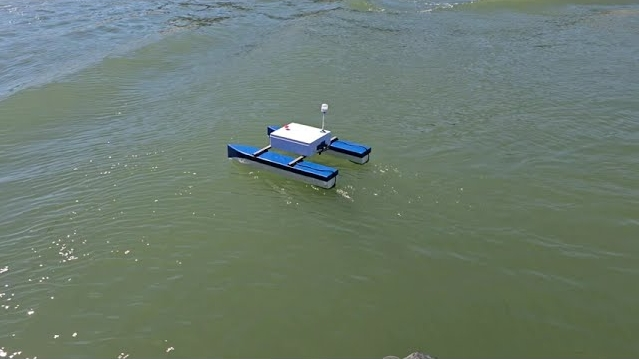
\includegraphics[width=0.5\linewidth]{thumbnail-youtube.jpg}};
            % Draw a red play button in the center
            \draw[fill=red, opacity=0.8] (0,0) circle [radius=0.7cm];
            \fill[white] (-0.25,0.35) -- (-0.25,-0.35) -- (0.4,0) -- cycle;
        \end{tikzpicture}%
    }
    \caption{Demonstração do \gls{usv} em funcionamento automático e manual (clique na imagem para abrir o vídeo no YouTube).}
    \label{fig:video-usv}
\end{figure}

\section{Sumário}

A estratégia de testes adotada demonstrou-se eficaz, permitindo a deteção e resolução de problemas de forma faseada e garantindo que o sistema final apresentava fiabilidade e robustez. Os testes unitários asseguraram a operação correta de cada módulo, os ensaios de integração confirmaram a coerência da arquitetura modular, e a validação em ambiente real comprovou a aplicabilidade do protótipo em cenários operacionais complexos. Em conjunto, estes resultados confirmam o cumprimento dos objetivos estabelecidos e a viabilidade da solução proposta para o controlo autónomo de veículos de superfície não tripulados.  
